\section{Status and Evaluation}
\label{sec:evaluation}

\subsection{Portability}
We have two proof-of-concept implementations, one over UDP Sockets and
one over Portals 3.3.

The Sockets prototype driver opens one SOCK\_DGRAM (UDP) socket per
CCI endpoint, with CCI  providing optional reliability and optional
ordering (UU, RO, RU). 
The Sockets driver multiplexes connections over a single socket.
Enough functions are complete including RMA write to allow simple ping pong
tests to exercise the CCI API.

The Portals implementation provides UU, RO, and RU over the portals
interface. Since Portals assumes a reliable interconnect, the
only difference between a CCI UU connection and a RO/RU connection is that we
complete a UU send when we receive the Portals' SEND\_END event which indicates
that the sender's buffer is no longer needed (i.e. the data is on the wire).
For a reliable connection, we report a completion when we get the Portals' ACK
of receipt at the peer.

\subsection{Performance}
We wrote a native Portals ping pong and compared it to the CCI ping pong
performance. We ran tests on a Cray XT6 and locked the processes to the same
cores for both tests. The CCI over Portals HRT ping pong
was less than 200ns more than the native Portals' performance up to 256 bytes.
For an eight byte message, for example, CCI's latency is 5.91\us versus 
5.74\us for native Portals. Figures \ref{fig:latency} and \ref{fig:bw} show latency
and bandwidth for active messages up to 8 KB on a Cray XT6.

\begin{figure}[htbp]
\centering
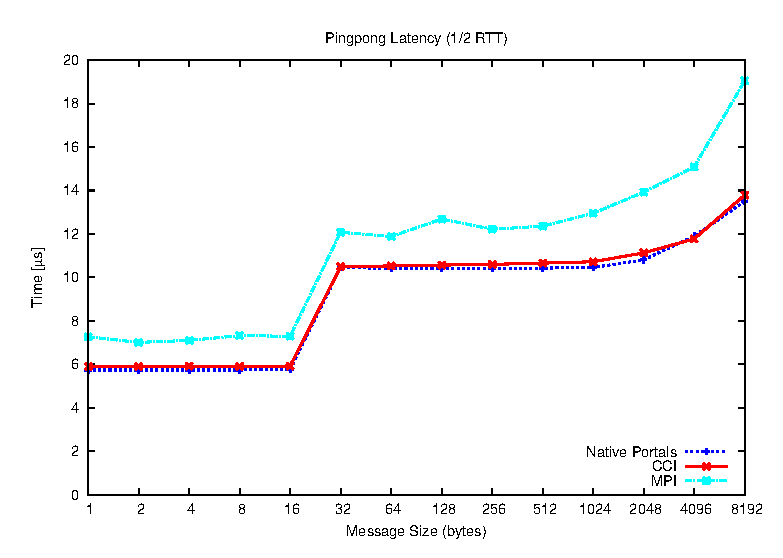
\includegraphics[width=3.45in]{pingpong-latency.eps}
\caption{Ping pong Latency when using Portals on SeaStar}
\label{fig:latency}
\end{figure}

\begin{figure}[htbp]
\centering
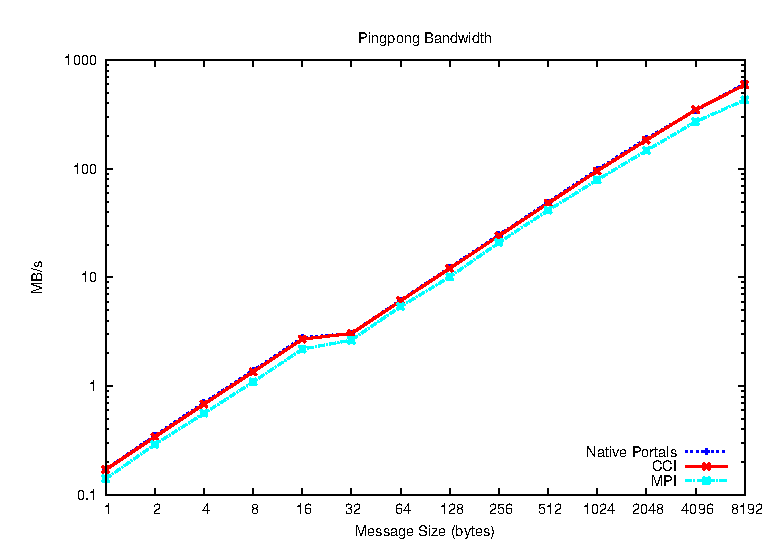
\includegraphics[width=3.45in]{pingpong-bw.eps}
\caption{Ping pong Bandwidth when using Portals on SeaStar}
\label{fig:bw}
\end{figure}

\begin{figure}[htbp]
\centering
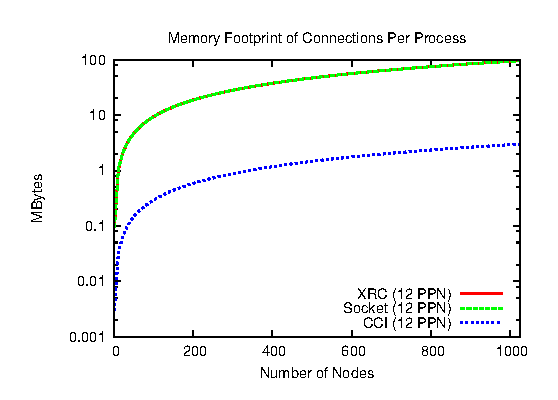
\includegraphics[width=3.45in]{memory_log.eps}
\caption{Memory footprint for connections per process}
\label{fig:memory}
\end{figure}

\subsection{Scalability}
CCI uses connection-oriented semantics with minimal per-connection resources.
For the Portals driver, each connection requires 104 bytes on 64-bit machines
(20 bytes for the public CCI connection struct, 20 bytes for the private CCI
struct, and 64 bytes for the Portals driver connection struct).  The sock driver
needs 140 bytes for each connection.

Figure \ref{fig:memory} illustrates the connection state for
Verbs, BSD Sockets, and CCI. Verbs memory usage scales
linearly~\cite{Shipman:2008:XIS:1431669.1431683} with the number of
connected peers when Reliable Connected (RC) mode. This is
the best case scenario for Verbs. The Sockets usage is derived from
the minimum 4 KB page send and receive buffers and internal state tied
to the connection. 

%% In addition to minimal connection state, CCI, Verbs, and Sockets
%% require additional memory for send/receive buffers. Both CCI and Verbs
%% support a shared memory pool model for send/receive buffers. 

The CCI usage conservatively assumes 256 bytes (assuming alingment padding,
etc.) as used in the UDP driver. Obviously, if CCI is implemented over Verbs,
for example, then this amount is on top of the underlying implementation. In
order to provide support for Verbs hardware (InfiniBand, iWARP, etc.), we intend
to use Verb's Unreliable Datagram (UD) mode to avoid the QP memory usage by
Verb's Reliable Connected (RC) or eXtended Reliable Connected (XRC) modes.

% LocalWords:  DGRAM UU RO RMA ACK XT RTT ns CCI's SeaStar struct alingment UD
% LocalWords:  Datagram QP eXtended
